%\chapter{Online Learning and Online Convex Optimisation}
\chapter{Online Learning}
\label{ch:ol}

\minitoc


%\emph{Online learning} represents an important family of machine learning algorithms, in which a learner attempts to perform an online prediction (or any type of decision-making) task by learning a model/hypothesis from a sequence of data instances one at a time. The goal of online learning is to ensure that the online learner would make a sequence of accurate predictions (or correct decisions) given the knowledge of correct answers to previous prediction or learning tasks, and possibly additional information. This is in contrast to many traditional \emph{batch} or \emph{offline} machine learning algorithms that are often designed to learn a model from the entire training data set at once.
%
%This chapter aims to provide a non-exhaustive survey of the online machine learning literature, through a systematic review of basic ideas and key principles. Generally speaking, based on the types of learning and feedback information, the existing online learning research can be classified into three major categories: (i) \emph{online supervised learning}, in which full feedback information is always available, (ii) \emph{online learning with limited feedback}, and (iii) \emph{online unsupervised learning}, where no feedback is available. Due to space constraints, this chapter will mainly focus on the first category.
%
%
%
%
\section{Introduction}
%
%Machine learning plays a crucial role in modern data analytics and artificial intelligence (AI) applications. Traditional machine learning paradigms often work in a batch, or offline, fashion (especially for supervised learning), where a model is learned from an entire training data set at once, to then be deployed for inference purposes on (previously unseen) subsequent data. Such learning methods suffer from expensive re-training cost when dealing with new datapoints, and thus are scale poorly in real-time applications. In the era of big data, traditional batch learning paradigms have become more and more restrictive, especially in situations where live data grows and evolves rapidly. Making machine learning scalable and practical for learning from continuous data streams has become an open grand challenge in machine learning and AI.
%
%Unlike traditional machine learning, \emph{online learning} includes an important family of learning techniques that are designed to learn models from data in a sequential manner. Online learning overcomes the drawbacks of traditional batch learning in that the underlying models can be updated instantly and efficiently when new training data arrives. Besides, online learning algorithms are often easy to understand, simple to implement, and often founded on solid theory with rigorous regret bounds. Along with the need to make machine learning practical for big data analytics, online learning has increasingly gained traction over recent years.
%
%This chapter seeks to provide a brief survey of the online learning literature. Online learning has been extensively studied across different fields, ranging from machine learning, data mining, statistics, optimisation and applied math, to AI and data science. Our aim here is to distill the core ideas of online learning methodologies and their applications, with a focus on online supervised learning.
%
%
%\subsection{What is online learning?}
%
%Traditional machine learning paradigm often runs in a batch learning fashion, e.g. a supervised learning task, where a collection of training data is given in advance to train a model. Such a paradigm requires the entire training data set to be made available prior to the learning task, and the training process is often done in an offline environment due to the expensive training cost. Traditional batch learning methods suffer from some critical drawbacks: (i) high computational overhead in terms of both time and space, and (ii) poor scalability for large-scale applications because the model often has to be re-trained from scratch for new training data.
%
%In contrast, online learning is naturally suited to data arriving in a sequential order, from which a learner aims to learn the best predictor for future datapoints at every timestep. Online learning is able to overcome the drawbacks of batch learning in that the predictive model can be updated instantly for any new data instances. Thus, online learning algorithms are far more efficient and scalable for large-scale machine learning in real-world data analytics tasks, in which the data are not only large in size, but also arrive at a high speed.
%
%
%\subsection{Tasks and applications}
%
%Similar to traditional (batch) machine learning methods, online learning techniques can be applied to solve a variety of tasks in a wide range of real-world application domains. Examples of online learning tasks include the following.
%
%\paragraph{Supervised learning tasks}
%
%Online learning algorithms can be derived for supervised learning tasks. One of the most common tasks is classification, aiming to predict the label of a new data instance, based on past instances whose labels are known. For example, a commonly studied task in online learning is online binary classification (e.g., spam email filtering) which only involves two categories (`spam' vs `benign' emails).
%%Other types of supervised classification tasks include multi-class classification, multi-label classification and multiple-instance classification.
%
%In addition to classification tasks, another common supervised learning task is regression analysis, which refers to the process of estimating relationships among variables (typically between a dependent variable and one or more independent variables). Online learning techniques are inherently appropriate for regression tasks, e.g. the analysis of financial time series, in which data are received in a sequential manner. Another closely related application is online
%portfolio selection, where a portfolio manager employs an online learning algorithm with the aim of finding a good (i.e., profitable and low-risk) strategy for making a sequence of asset allocation decisions.
%
%
%\section{Online Supervised Learning}
%
%\subsection{Problem setting}
%
%
%
%Without loss of generality, we give a formal formulation of online binary classification, perhaps the most classic online learning problem. On each round, a learner receives a data instance, and then makes a prediction for the label, or class, of that instance. Thereafter, the learner receives the true label from the environment. Based on that feedback, the learner can measure the loss incurred due to the discrepancy between her prediction and the true answer. Finally, the learner uses that information to update her predi
%
%\subsection{Overview}
%
%\subsection{First-order online learning}

Online learning \citep{lugosi, shalev-shwartz11, oco} represents an important family of efficient and scalable algorithms for time-aware and large-scale applications. In general, these algorithms are fast, simple and based only on a handful of statistical assumptions, making them applicable to a wide range of settings. Online methods have therefore rapidly gained traction in the field of big data analytics, where avoiding processing extremely large batches of data is important.

Online learning has been actively studied in several communities, including machine learning/artificial intelligence, statistics and game theory. Over the past years, a variety of online algorithms have been proposed. To a large extent, the design of these algorithms has been influenced by convex optimisation tools, whence their release under the umbrella of \emph{online convex optimisation}. So far, however, the vast majority of these techniques are frequentist: they make point rather than probabilistic predictions, thus failing to account for model/prediction uncertainty. Furthermore, they rely on a few hyperparameters that must be hand-picked, which renders their predictive performance sensitive to specific hyperparameter configurations. This motivates a Bayesian approach to online learning that explicitly takes model/prediction uncertainty into account, and simultaneously enables automatic hyperparameter tuning by letting the data speak for themselves, which is precisely the raison d'\^{e}tre of this thesis.

%Before diving in, however, it is helpful to review the existing literature that will serve as a building block for the methods developed herein. To this end, this chapter contains a brief survey of the relevant, so-called \emph{first-order} and \emph{second-order} online learning algorithms for linear regression --- our main focus throughout this thesis. The survey here is inspired by \citep{ol-survey}, which may be referred to for a deeper treatment of online learning.
\begin{mccorrection}
Before diving in, however, it is helpful to review the existing literature that will serve as a building block for the methods developed herein. To this end, this chapter contains a brief survey of the relevant, so-called \emph{first-order} and \emph{second-order} online learning algorithms for linear regression --- our main focus throughout this thesis. The survey here largely follows the publications of \citep{hoi-ol-tutorial} and \citep{ol-survey}, which may be referred to for a deeper treatment of online learning.
\end{mccorrection}
%We shall begin by outlining the differences between the offline and online learning paradigms (and under which circumstances the latter is preferable), followed by an overview of the wide range of applications of online learning. We shall conclude by highlighting the shortcomings of the reviewed algorithms, and how our proposed framework aims to overcome these.

\subsection{Online vs offline learning}

The traditional learning paradigm in machine learning and related disciplines is \emph{offline learning}, also known as \emph{batch learning}. Perhaps the main building block of offline learning is the assumption that the data are \emph{stationary}, which justifies training a model once, on a batch of data, and repeatedly using it on subsequent observations.

Alas, in many real-world time-series applications, the underlying data generating mechanism keeps changing over time, thereby violating the assumption of stationarity. In this case, offline algorithms need to be retrained every time a new datum is made available to them. This can be highly inefficient and can introduce costly delays in the decision-making process, particularly in time-aware applications, such as algorithmic trading where the data streams used as inputs by the learning machine may
be imported at very high sampling frequencies (e.g. every minute or less) \citep{montana}. Moreover, in large-scale applications, the dimensionality of the data makes it impossible to store them after they have been processed, due to the practical bounds on memory utilisation \citep{domingos}.

\begin{mccorrection}
There a few additional reasons why online learning is different from offline/batch learning, namely:
\begin{itemize}
\item ˆ Offline/batch methods do not learn by minimising (static or dynamic) regret. They are based on alternative optimisation criteria, such as empirical risk minimisation or maximum likelihood estimation. That is why even when performed on a sliding- or rolling-window basis, most offline methods do not fall under the umbrella of `online learning' technically speaking, albeit in practice, they can indeed be utilised for learning of time series data online, except perhaps in the circumstances outlined in the two bullet points below.
\item The environment against which an online learner plays can be \emph{adversarial}, meaning the losses the learner receives from the environment are time-varying and cannot be known in advance (as the environment reveals them only \emph{after} the online learner has played her action).
\item The feedback obtained from the environment in online learning can be \emph{partial} rather than complete, meaning that at each round after the online learner has chosen her action $\mathbf{w}_t$, the environment does not reveal the entire loss function $\ell_t(\cdot)$, but only the gradient thereof at $\mathbf{w}_t$ or the loss value incurred $\ell_t(\mathbf{w}_t)$ at the chosen weights such as in the bandit setting (this partial feedback may even be noisy). 
\end{itemize}
Having said that, it is worthwhile noting that the term `online learning' exists in other communities outside the OCO and no-regret community.%, for example in the Bayesian filtering literature.
\end{mccorrection}

As a result, in real-time forecasting applications, one often prefers online to offline learning, due to its numerous competitive advantages which, for completeness, are listed below:
\begin{itemize}
	\item Avoid retraining when adding new examples;
	\item Fast, low memory footprint;
	\item Strong adaptability to changing environments;
	\item Simple to implement;
	\item Easy to be parallelised;
	\item Theoretical guarantees;
	\item Can be converted to batch learning.
\end{itemize}


\subsection{Applications of online learning}

For the aforementioned reasons, online learning is the favourite learning paradigm in streaming environments. Over recent years, it has gained considerable traction in big data mining. Further areas of application are depicted in Figure~\ref{fig:online-learning-applications}.
\begin{figure}[H]
	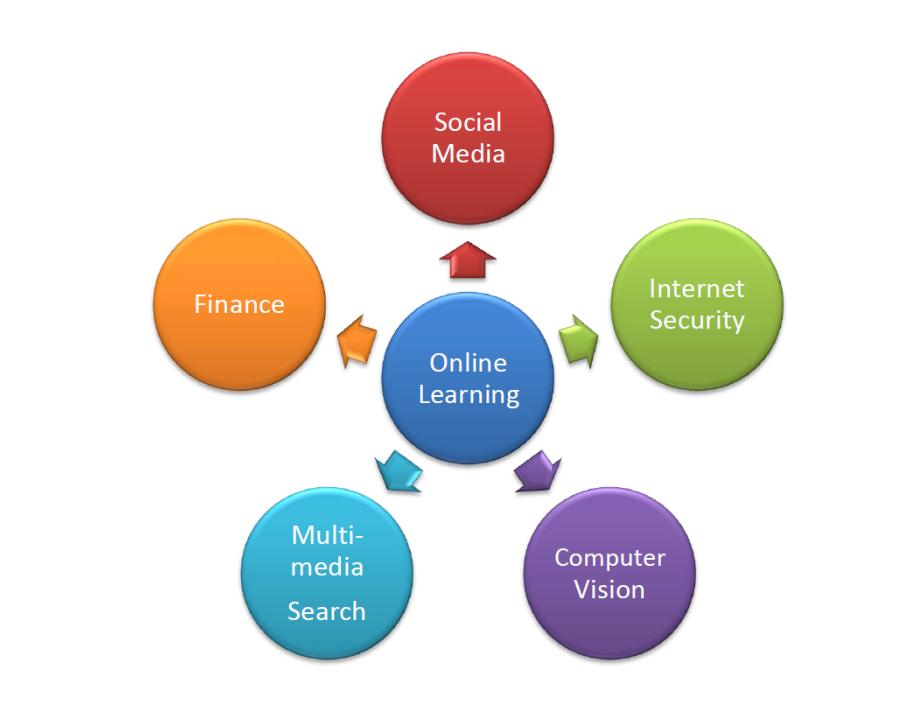
\includegraphics[width=\textwidth, height=\textheight, keepaspectratio]{online-learning-applications}
	\caption{Some areas of application of online learning. Source: \citep{hoi-ol-tutorial}.}
	\label{fig:online-learning-applications}
\end{figure}

Starting with social media, online learning is employed as a mining tool for social media streams to gather business intelligence, such as public emotion and product/brand sentiment. In internet security, it is used as an online anomaly detection mechanism, ranging from spam email detection to the identification of fraudulent credit card transactions. In computer vision, it enables real-time object tracking for video surveillance purposes, especially for the detection of anomalous events from realtime video streams. On the other hand, interactive image/video search via online relevance feedback is one of the various applications of online learning to multimedia search. Finally, in finance, online portfolio selection has recently been demonstrated to outperform traditional benchmarks \citep{olps-survey}. As we already hinted, online methods are crucial in this field, as sequential decisions need to be promptly taken regarding the allocation of wealth among different assets.




\section{Problem Statement and Related Theory}

We first give a formal formulation of online linear regression, which will be our main subject of focus throughout this thesis, and then introduce the basics of statistical learning theory and online convex optimisation as the theoretical foundations for online learning techniques.


\subsection{Online linear regression}

Online learning operates on a sequence of data examples with timestamps. At each step $t$, the learner receives an instance $\mathbf{x}_t \in \mathbb{R}^n$. It first attempts to make a prediction for the output of the incoming instance which, in the case  of linear regression, takes the form $\hat{y}_t = \mathbf{w}_t^\text{T} \mathbf{x}_t$, where $\mathbf{w}_t \in \mathbb{R}^n$ is the incrementally learned weight vector. After making the prediction, the true output $y_t \in \mathbb{R}$ is revealed, and the learner then computes the incurred loss $\ell(y_t, \hat{y}_t) \in \mathbb{R}_{\geq 0}$, based on some criterion to measure the difference between the learner’s prediction and the revealed true output. Using this loss, the learner finally decides whether and how to update the regression model at the end of each learning step.

The following algorithmic framework gives an overview of most first-order online learning algorithms for linear regression, where $\Delta(\mathbf{w}_t; (\mathbf{x}_t, y_t))$ denotes the update of the regression models. Different online learning algorithms operate under different definitions, and designs of the loss function $\ell(\cdot)$ and the updating function $\Delta(\cdot)$.
\begin{algorithm}[H]
  \caption{Online learning framework for linear regression}
\label{alg:online-linear-regression}
  \begin{algorithmic}[1]
    \STATE {\bfseries Initialisation:} $\mathbf{w}_1 = \mathbf{0}_{n\times 1}$
    \FOR{$t=1, 2, \ldots, T$}
      \STATE the learner receives an incoming instance $\mathbf{x}_t \in \mathbb{R}^n$
      \STATE the learner predicts the output: $\hat{y}_t = \mathbf{w}_t^\text{T} \mathbf{x}_t$
      \STATE the true output is revealed by the environment: $y_t \in \mathbb{R}$
      \STATE the learner calculates the suffered loss: $\ell(\mathbf{w}_t; (\mathbf{x}_t, y_t))$
    \IF{$\ell(\mathbf{w}_t; (\mathbf{x}_t, y_t)) > 0$}
      \STATE the learner updates the regression model according to
      \begin{equation*}
      	\mathbf{w}_{t+1} = \mathbf{w}_t + \Delta(\mathbf{w}_t; (\mathbf{x}_t, y_t))
      \end{equation*}
    \ENDIF
    \ENDFOR
  \end{algorithmic}
\end{algorithm}
%By running such an algorithm over a sequence of $T$ rounds, the cumulative loss achieved by the algorithm can be measured as $L_T = \sum_{t=1}^T \ell(y_t, \hat{y}_t)$. The classic goal in an online learning task is to minimise the regret of the underlying online learner's predictions against the best fixed model in hindsight, i.e.\
%\begin{equation}
%	R_T = \sum_{t=1}^T \ell(y_t, \mathbf{w}_t^\text{T} \mathbf{x}_t) - \min_{\mathbf{w}} \sum_{t=1}^T \ell(y_t, \mathbf{w}^\text{T} \mathbf{x}_t),
%\end{equation}
%where the second term is the loss suffered by the optimal model $\mathbf{w}^*$, which can only be known in hindsight after seeing all the instances and their corresponding targets. From the theoretical perspective of regret minimisation, if an online algorithm guarantees that its regret is sublinear as a function of $T$, i.e.\ $R_T = o(T)$, it also satisfies the condition $\lim_{T \rightarrow \infty} R(T)/T = 0$, meaning that on average, the learner performs almost as well as the best fixed model in hindsight.
\begin{mccorrection}
By running such an algorithm over a sequence of $T$ rounds, the cumulative loss achieved by the algorithm can be measured as $L_T = \sum_{t=1}^T \ell(y_t, \hat{y}_t)$. The classic goal in an online learning task is to minimise the regret of the underlying online learner's predictions against the best fixed model in hindsight, i.e.\
\begin{equation}
	R_T = \sum_{t=1}^T \ell(y_t, \mathbf{w}_t^\text{T} \mathbf{x}_t) - \min_{\mathbf{w}} \sum_{t=1}^T \ell(y_t, \mathbf{w}^\text{T} \mathbf{x}_t),
\end{equation}
where the second term is the loss suffered by the optimal model $\mathbf{w}^*$, which can only be known in hindsight after seeing all the instances and their corresponding targets. From the theoretical perspective of regret minimisation, the notion of \emph{no regret} means $R_T \leq b(T)$, where $b(T)$ in $o(T)$.
\end{mccorrection}

\subsection{Statistical learning theory}

Statistical learning theory, first introduced in the late 1960's, is one of key foundations for the theoretical analysis of machine learning problems, especially for supervised learning. There are many comprehensive survey articles and books on the subject matter, including the seminal work of Vladimir Vapnik \citep{vapnik98, vapnik99}. In the following, we review some basic concepts.

\subsubsection{Empirical error minimisation}

Assume instance $\mathbf{x}_t$ is generated randomly from a fixed but unknown distribution $P(\mathbf{x})$, and that the corresponding output $y$ is also generated from a fixed but unknown distribution $P(y|\mathbf{x})$. The joint distribution of the data is then $P(\mathbf{x}, y) = P(\mathbf{x}) P(y|\mathbf{x})$. The goal of supervised learning is to find a prediction function $f(\mathbf{x})$ that minimises the expected value of the loss function
\begin{equation}
	R(f) = \int \ell(y, f(\mathbf{x})) \, \mathrm{d} P(\mathbf{x}, y),
\end{equation}
also termed the \emph{true risk} functional. The solution $f^* = \argmin R(f)$ is the optimal predictor.

In general, the true risk functional cannot be computed directly because of the unknown distribution $P(\mathbf{x}, y)$. In practice, we approximate it by estimating the risk over a finite collection of examples $(\mathbf{x}_1, y_1), \ldots, (\mathbf{x}_m, y_m)$, drawn in an i.i.d. fashion. This estimated risk is known as \emph{empirical risk} or \emph{empirical error}, and is given by
\begin{equation}
	R_\text{emp}(f) = \frac{1}{m} \sum_{i=1}^m \ell(y_i, f(\mathbf{x}_i)).
\end{equation}
Learning via empirical risk minimisation (ERM) consists in finding a hypothesis $f$ over a hypothesis space $\mathcal{F}$ by solving
\begin{equation}
	\hat{f}_m = \argmin_{f\in\mathcal{F}} \; R_\text{emp}(f).
\end{equation}
ERM forms the theoretical basis for many machine learning algorithms. In the case of regression, assuming $\mathcal{F}$ is the set of linear regressors and the squared loss is used, the ERM principle suggests that the best linear model $\mathbf{w}^*$ can be learned by minimising the following objective with respect to $\mathbf{w}$:
\begin{equation}
	R_\text{emp}(\mathbf{w}) =  \frac{1}{m} \sum_{i=1}^m (y_i - \mathbf{w}^\text{T}\mathbf{x}_i)^2.
\end{equation}

\subsection{Convex optimisation theory}

Many online learning problems can essentially be (re-)formulated as an online convex optimisation (OCO) task. In the following, we introduce some of the basics of OCO.

An online convex optimisation task typically consists of two major elements: a convex set $\mathcal{S}$ and a convex loss function $\ell_t(\cdot)$. At each time step $t$, the online algorithm picks a weight vector $\mathbf{w}_t \in \mathcal{S}$, after which it suffers a loss $\ell_t(\mathbf{w}_t)$. The goal of the online algorithm is to play a sequence of decisions $\mathbf{w}_1, \mathbf{w}_2, \ldots$ so as to minimise the regret in hindsight.

More formally, an online algorithm aims to achieve a low regret $R_T$ after $T$ rounds, where the regret $R_T$ is defined as
\begin{equation}
\label{eq:regret}
	R_T = \sum_{t=1}^T \ell_t(\mathbf{w}_t) - \inf_{\mathbf{w}^* \in \mathcal{S}} \sum_{t=1}^T \ell_t(\mathbf{w}^*).
\end{equation}
In an online linear regression task on a sequence of examples $(\mathbf{x}_t, y_t)$, $t=1,\ldots,T$, with $\mathbf{x}_t \in \mathbb{R}^n$ and $y_t \in \mathbb{R}$, a commonly used loss function is the squared loss $\ell_t(\mathbf{w}) = (y_t - \mathbf{w}^\text{T}\mathbf{x}_t)^2$. In this case, the convex set $\mathcal{S}$ would be $\mathbb{R}^n$. There are a variety of algorithms to solve this problem.

Below, we briefly discuss two major families of OCO methods, namely first-order and second-order algorithms that will play an instrumental role in the development of our research work. For a comprehensive treatment of the subject, the interested reader is referred to the books by \citet{shalev-shwartz11, oco}.

\section{First-Order Online Learning}

\begin{mccorrection}
First-order methods aim to minimise the regret in Eq. \eqref{eq:regret} using first-order gradient information. The majority of first-order algorithms are classification algorithms. Only a few have been developed for regression tasks, such as online gradient descent \citep{ogd} and online passive-aggressive regression \citep{crammer06}. We describe these below.
\end{mccorrection}

\subsection{Online passive-aggressive regression}

Online passive-aggressive (PA) regression is a popular online regression algorithm that was introduced in \citep{crammer06}. It has been applied across a number of diverse areas, including online portfolio selection \citep{pamr}, non-negative matrix factorisation and completion \citep{blondel14}, and statistical machine translation \citep{turchi}.

On every round, the PA regression algorithm receives an instance $\mathbf{x}_t$ and predicts a target value $\hat{y}_t = \mathbf{w}_{t}^\text{T}\mathbf{x}_t$ using its internal regression function. After making a prediction, the algorithm is given
the true target value $y_t$ and suffers an instantaneous loss. PA regression relies on the $\epsilon$-insensitive loss function (ILF) \citep{vapnik98}, defined as
\begin{equation}
\label{eq:ilf}
	 \ell_{\epsilon}(\mathbf{w}; \mathbf{z}) \equiv
	 \begin{cases}
	 	0 & \text{if } |y - \mathbf{w}^\text{T}\mathbf{x}| \leq \epsilon \\
	 	|y - \mathbf{w}^\text{T}\mathbf{x}| - \epsilon & \text{otherwise}
	 \end{cases},
\end{equation}
where $\mathbf{z} = (\mathbf{x}, y)$ and $\epsilon$ is a positive hyperparameter that controls the algorithm's sensitivity to prediction mistakes. The ILF is zero when the predicted target deviates from the true target by less than $\epsilon$ units, and otherwise grows linearly with $|y_t - \hat{y}_t|$. At the end of every round, the algorithm uses $\mathbf{w}_t$ and the example $\mathbf{z}_t$ to generate a new weight vector $\mathbf{w}_{t+1}$, which is then used to extend the prediction on the next round.

We now describe how the PA regression algorithm sequentially updates its weight vector. The latter is initialised to the zero vector. Then, on each subsequent round, the algorithm sets the new weight vector to be
\begin{equation}
\label{eq:generic-pa-optpb}
	\mathbf{w}_{t+1} = \argmin_{\mathbf{w} \in \mathbb{R}^n} \; \frac{1}{2}\Vert\mathbf{w} - \mathbf{w}_t\Vert_2^2
	\qquad \text{s.t.} \qquad \ell_{\epsilon}(\mathbf{w}; \mathbf{z}_t) = 0.
\end{equation}
The set $C_{\epsilon}(\mathbf{z}_t) \equiv \{\mathbf{w} \in \mathbb{R}^n : \ell_{\epsilon}(\mathbf{w}; \mathbf{z}_t) = 0\}$ is a hyper-slab of width $2\epsilon$. Geometrically, the PA algorithm for regression projects $\mathbf{w}_t$ onto this hyper-slab at the end of every round, unless $\mathbf{w}_t$ suffers no loss from the new data, i.e.\ $\mathbf{w}_t \in C_{\epsilon}(\mathbf{z}_t)$. These mechanics are illustrated in Figure~\ref{fig:pa-illustration}.
\begin{figure}[t]
	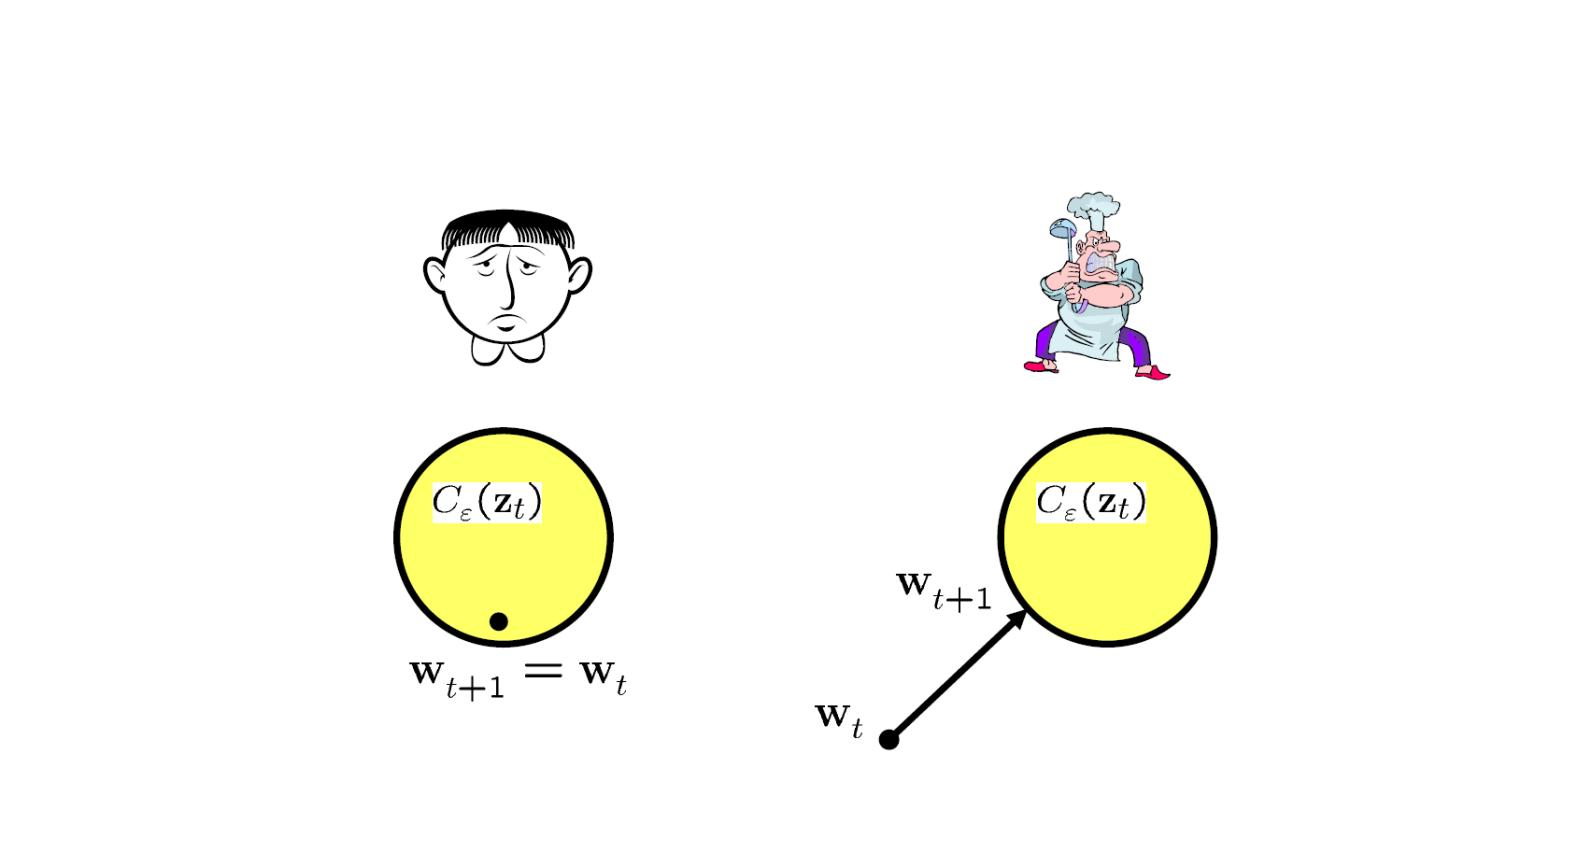
\includegraphics[width=\textwidth, height=\textheight, keepaspectratio]{pa-illustration}
	\caption{The mechanics of linear PA regression. The algorithm \emph{passively} assigns $\mathbf{w}_{t+1} = \mathbf{w}_t$ as long as $\mathbf{w}_t$ incurs no loss on the incoming example $\mathbf{z}_t$. Otherwise, it \emph{aggressively} projects $\mathbf{w}_t$ onto the feasible set $C_{\epsilon}(\mathbf{z}_t)$ of weight vectors which attain zero loss. Source: \url{https://home.ttic.edu/~shai/ppt/PassiveAggressive.ppt}.}
	\label{fig:pa-illustration}
\end{figure}

Using the shorthand $\ell_t = \ell_{\epsilon}(\mathbf{w}; \mathbf{z}_t)$, \citet{crammer06} showed that the update in Eq. \eqref{eq:generic-pa-optpb} has a closed-form solution, namely
\begin{equation}
\label{eq:generic-pa-update-rule}
	\mathbf{w}_{t+1}
	= \mathbf{w}_t + \tau_t\mathbf{v}_t,
\end{equation}
where $\tau_t = \ell_t / \Vert\mathbf{x}_t\Vert_2^2$ is the Lagrange multiplier associated with the feasibility constraint $\mathbf{w}_{t+1} \in C_{\epsilon}(\mathbf{z}_t)$, and $\mathbf{v}_t \equiv \mathrm{sgn}(y_t - \hat{y}_t)\mathbf{x}_t$ represents the direction of the update.

\subsubsection{Soft-margin PA regression}

As discussed above, the PA algorithm employs an aggressive update strategy, by modifying the weight vector by as much as needed to satisfy the constraint imposed by the current example. In certain real-life situations, this strategy may also result in undesirable consequences. Consider for instance the common phenomenon of outliers. An outlier may cause the PA algorithm to drastically change its weight vector in the wrong direction. A single outlier may thereby lead to several prediction mistakes on subsequent rounds.

To cope with such problems, \citet{crammer06} developed two variations on the PA update that employ gentler update strategies. These variations are based on the technique previously used to derive soft-margin classifiers \citep{vapnik98}: they introduce a non-negative slack variable $\xi$ into the optimisation problem defined in Eq. \eqref{eq:generic-pa-optpb}. This variable can be introduced in two different ways. First, we consider the update where the objective function scales linearly with $\xi$:
\begin{equation}
\label{eq:paI-optpb}
	\mathbf{w}_{t+1} = \argmin_{\mathbf{w},\, \xi} \; \Big\{\frac{1}{2}\Vert\mathbf{w} - \mathbf{w}_t\Vert_2^2 \, + \, C\xi\Big\}
	\qquad \text{s.t.} \qquad \ell_{\epsilon}(\mathbf{w}; \mathbf{z}_t) \leq \xi \quad \text{and} \quad \xi \geq 0.
\end{equation}
Here, $C$ is a positive parameter which controls the influence of the slack term on the objective function. Specifically, larger values of $C$ imply a more aggressive update, and $C$ is therefore referred to as the \emph{aggressiveness parameter} of the algorithm. This variant of PA regression is known as \emph{PA-I}.

Alternatively, the objective function scales quadratically with $\xi$, resulting in the following constrained optimisation problem:
\begin{equation}
\label{eq:paII-optpb}
	\mathbf{w}_{t+1} = \argmin_{\mathbf{w},\, \xi} \; \Big\{\frac{1}{2}\Vert\mathbf{w} - \mathbf{w}_t\Vert_2^2 \, + \, C\xi^2\Big\}
	\qquad \text{s.t.} \qquad \ell_{\epsilon}(\mathbf{w}; \mathbf{z}_t) \leq \xi.
\end{equation}
Note that the constraint $\xi \geq 0$ which appears in Eq. \eqref{eq:paI-optpb} is no longer necessary, since $\xi^2$ is always non-negative. The algorithm that results from this update is termed \emph{PA-II}. As with PA-I, $C$ is a positive
parameter which governs the extent to which the PA-II update is aggressive.

As shown in \citep{crammer06}, the updates of PA-I and PA-II share the simple analytical solution $\mathbf{w}_{t+1} = \mathbf{w}_t + \tau_t \mathbf{v}_t$, as defined in Eq. \eqref{eq:generic-pa-update-rule}, but with the following Lagrange multipliers, respectively:
\begin{equation}
	\tau_t = \min\bigg\{C, \; \frac{\ell_t}{\Vert\mathbf{x}_t\Vert_2^2}\bigg\} \quad (\text{PA-I})
	\qquad \text{and} \qquad
	\tau_t = \frac{\ell_t}{\Vert\mathbf{x}_t\Vert_2^2 \, + \, \frac{1}{2C}} \quad (\text{PA-II}).
\end{equation}
All PA variants are outlined in Algorithm~\ref{alg:pa}.
\begin{algorithm}[H]
  \caption{Passive-Aggressive Algorithms}
\label{alg:pa}
  \begin{algorithmic}[1]
    \STATE {\bfseries Initialisation:} $\mathbf{w}_1 = \mathbf{0}_{n\times 1}$, insensitivity parameter $\epsilon \geq 0$, aggressiveness parameter $C > 0$
    \FOR{$t=1, 2, \ldots, T$}
      \STATE receive $\mathbf{x}_t \in \mathbb{R}^n$, predict $\hat{y}_t$ using $\mathbf{w}_t$
      \STATE suffer loss $\ell_t(\mathbf{w}_t)$
      \STATE set
      \begin{equation*}
      	\tau_t = 
      	\begin{cases}
      		\ell_t / \Vert\mathbf{x}_t\Vert_2^2 & \text{(PA)} \\
      		\min\{C,\, \ell_t / \Vert\mathbf{x}_t\Vert_2^2\}  & \text{(PA-I)} \\
      		\frac{\ell_t}{\Vert\mathbf{x}_t\Vert_2^2 \, + \, \frac{1}{2C}} & \text{(PA-II)} \\
      	\end{cases}
      \end{equation*}
    \STATE update $\mathbf{w}_{t+1} = \mathbf{w}_t + \tau_t \mathbf{v}_t$, where $\mathbf{v}_t = \mathrm{sgn}(y_t - \hat{y}_t)\mathbf{x}_t$
    \ENDFOR
  \end{algorithmic}
\end{algorithm}
%\paragraph{Relationship between PA-I and support vector regression}
%
%It is worthwhile noting that the PA-I optimisation problem in Eq. \eqref{eq:paI-optpb} is analogous to that which arises in $\epsilon$-support vector regression (SVR) \citep{vapnik98}. Indeed, the core of its construction can be viewed as finding a linear SVR on a single example, while replacing the norm constraint of SVR with a proximity constraint to the current weight vector.

\subsection{Online gradient descent}

As we mentioned earlier, many online learning problems can be formulated as an online convex optimisation (OCO) task, which can be solved by applying the online gradient descent (OGD) algorithm. The latter is perhaps the simplest algorithm that applies to the most general OCO setting. Based on standard gradient descent from offline optimisation, it was introduced in its online form by Martin Zinkevich \citep{ogd}. The pseudo-code for the algorithm is given in Algorithm~\ref{alg:ogd}.
\begin{algorithm}[H]
  \caption{Online Gradient Descent}
\label{alg:ogd}
  \begin{algorithmic}[1]
    \STATE {\bfseries Initialisation:} convex set $\mathcal{K}$, horizon $T$, $\mathbf{x}_1 \in \mathcal{K}$, learning-rate schedule $\{\eta_t\}$
    \FOR{$t=1, 2, \ldots, T$}
      \STATE play $\mathbf{x}_t$ and observe cost $f_{t}(\mathbf{x}_t)$
      \STATE update and project:
      \begin{align*}
      	\mathbf{y}_{t+1} &= \mathbf{x}_t - \eta_t \nabla f_{t}(\mathbf{x}_t) \\
      	\mathbf{x}_{t+1} &= \Pi_{\mathcal{K}}(\mathbf{y}_{t+1}) \equiv \argmin_{\mathbf{x} \in \mathcal{K}} \; \Vert\mathbf{x} - \mathbf{y}_{t+1}\Vert_2
      \end{align*}
    \ENDFOR
  \end{algorithmic}
\end{algorithm}

At each iteration, the algorithm takes a step from the previous point in the direction of the gradient of the previous cost. This step may result in a point outside of the underlying convex set. In such cases, the algorithm projects the point back onto the convex set, i.e.\ finds its closest point in the convex set. Despite the fact that the next cost function may be completely different from the costs observed thus far, the regret attained by the algorithm is sublinear (see \citep[Theorem~3.1.]{oco}). A conceptual illustration of the algorithm is given in Figure~\ref{fig:ogd}.
\begin{figure}[t]
	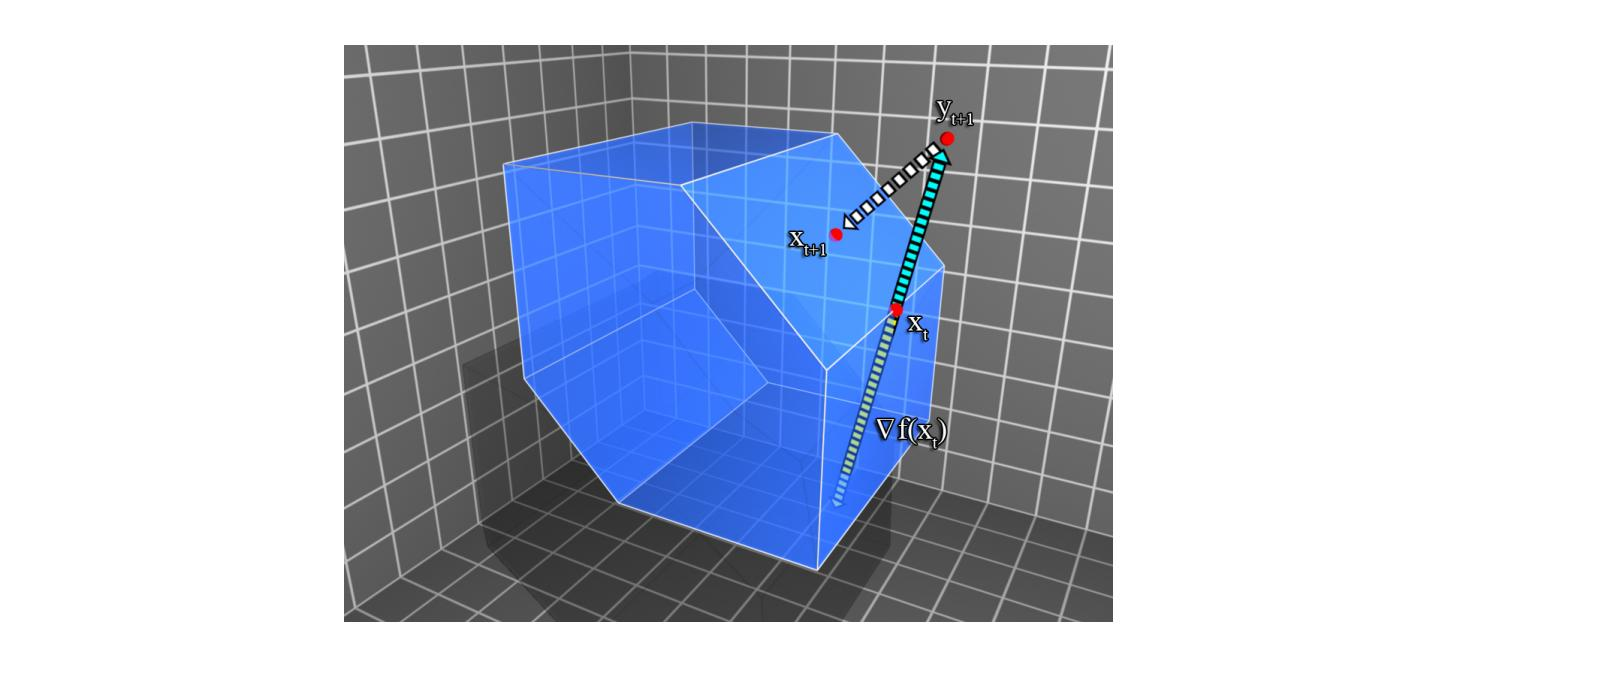
\includegraphics[width=\textwidth, height=\textheight, keepaspectratio]{ogd}
	\caption{Online gradient descent: the iterate $\mathbf{x}_{t+1}$ is derived by moving $\mathbf{x}_t$ into the direction of the current gradient $\nabla f_t(\mathbf{x}_t)$, then projecting it back onto $\mathcal{K}$. Source: \citep{oco}.}
	\label{fig:ogd}
\end{figure}

In the case of linear regression with a squared loss function, the update rule for OGD takes the form
\begin{equation}
	\mathbf{y}_{t+1} = \mathbf{x}_t - 2\eta_t (\hat{y}_t - y_t)\mathbf{x}_t.
\end{equation} 
In general, this rule is straightforward to implement, and takes linear time. OGD and PA share similar update rules, but differ in that OGD often employs some predefined learning-rate scheme, whereas PA chooses the optimal learning rate $\tau_t$ at each round (albeit subject to a predefined cost parameter $C$).
%In the literature, different OGD variants have been proposed to improve either theoretical bounds or practical issues, such as adaptive OGD (Hazan et al., 2007b), and mini-batch OGD (Dekel et al., 2012), amongst others. 




\section{Second-Order Online Learning}

%Unlike first-order online learning algorithms which only exploit the first-order information contained in the gradient for the purpose of solving online optimisation tasks, second-order online learning algorithms exploit both first-order and second-order information in order to speed up convergence. Despite their superior learning performance, a major drawback of second-order algorithms is their higher computational complexity. In what follows, we briefly describe some popular second-order online learning algorithms.

To improve the efficacy of first-order learning methods, recent years have witnessed the active development of second-order online learning algorithms. In general, these algorithms place a Gaussian prior distribution over the weights, with mean vector $\boldsymbol{\mu} \in \mathbb{R}^n$ and covariance matrix $\boldsymbol{\Sigma} \in \mathbb{R}^{n \times n}$. The model parameters are updated in the online learning process.

Examples of second-order algorithms for linear regression include adaptive regularisation of weight vectors \citep{arow}, which was inspired by confidence-weighted learning \citep{dredze08}, and a more recently introduced Bayesian treatment of online PA learning, namely online Bayesian passive-aggressive learning \citep{bayespa}.

\subsection{Confidence-weighted learning}

Confidence-weighted (CW) learning was introduced in \citep{dredze08} as a probabilistic extension of online passive-aggressive learning that takes into account model/parameter uncertainty by maintaining a probabilistic measure of confidence in each weight. Less confident weights are updated more aggressively than more confident ones. Weight confidence is formalised with a Gaussian distribution over weight vectors, which is updated for each new training instance so that the probability of correct classification for that instance under the updated distribution meets a specified confidence.

In the CW framework, the linear classifier is modelled with a Gaussian distribution, i.e.\ $\mathbf{w} \sim \mathcal{N}(\boldsymbol{\mu},\, \boldsymbol{\Sigma})$. Given an instance $\mathbf{x}$, the label is then predicted according to the sign of $\mathbf{w}^\text{T}\mathbf{x}$. The multivariate Gaussian distribution over weight vectors induces a univariate Gaussian distribution over the margin viewed as a random variable. Specifically:
\begin{equation}
	M \equiv y(\mathbf{w}^\text{T}\mathbf{x}) \sim \mathcal{N}(y(\boldsymbol{\mu}^\text{T}\mathbf{x}),\, \mathbf{x}^\text{T}\boldsymbol{\Sigma}\mathbf{x}).
\end{equation}


Following the intuition underlying the PA algorithms, the CW algorithm chooses the distribution closest in the KL divergence sense to the current distribution $\mathcal{N}(\boldsymbol{\mu}_t,\, \boldsymbol{\Sigma}_t)$. Thus, on round $t$, the algorithm sets the parameters of the distribution by solving the following convex optimisation problem:
\begin{align}
	\mathcal{N}(\boldsymbol{\mu}_{t+1},\, \boldsymbol{\Sigma}_{t+1})
	&= \min \quad \mathrm{KL}\big[\mathcal{N}(\boldsymbol{\mu},\, \boldsymbol{\Sigma}) \, \Vert \, \mathcal{N}(\boldsymbol{\mu}_t,\, \boldsymbol{\Sigma}_t)\big]
	\\ \nonumber
	& \text{s.t.} \qquad \mathbb{P}\Big\{y_{t}(\mathbf{w}^\text{T}\mathbf{x}_{t}) \geq 0\Big\} \geq \eta.
\end{align}
In plain English, this means that the new distribution should remain as close as possible to the previous distribution so that the classifier does not forget the information learnt from previous instances. The constraint reflects the fact that the new classifier should classify the new instance $\mathbf{x}_t$ correctly with probability higher than a predefined threshold parameter $\eta \in (0, 1)$.

Note that this is only the basic form of confidence weighted algorithms and has several drawbacks: i) similar to the hard-margin PA algorithm, the constraint forces the new instance to be correctly classified, which makes this algorithm very sensitive to noise; ii) the constraint is expressed in terms of a probability. It is easy to solve a problem with a constraint of the form $g(\boldsymbol{\mu}, \boldsymbol{\Sigma}) < 0$. However, a problem with a constraint on a probability is only solvable when the distribution is known. Thus, this method is hardly generalisable to other online learning tasks for which the constraint does not follow a Gaussian distribution.

\subsection{Adaptive regularisation of weights}

Confidence-weighted algorithms have been shown to perform well in practice (see, e.g., \citep{dredze08}), but they suffer from several problems. First, the update is quite aggressive, forcing the probability of predicting each example correctly to be at least $\eta > 1/2$ regardless of the cost to the objective. This may cause severe over-fitting when labels are noisy, especially considering the fact that the CW framework assumes that the data are linearly separable. Second, they are designed for classification, and it is not clear how to extend them to alternative settings such as regression. This is in part because the constraint is written in discrete terms where the prediction is either correct or no.

Adaptive regularisation of weights (AROW) is a variant of CW that was proposed by \citet{arow} to deal with both of the aforementioned issues, coping more effectively with label noise and generalising the advantages of CW learning in an extensible way. Like CW, AROW maintains a Gaussian distribution over weight vectors, with mean $\boldsymbol{\mu}$ and covariance $\boldsymbol{\Sigma}$. However, it expresses the CW constraint in terms of a set of regularisers, minimising the following unconstrained objective on each round:
\begin{equation}
	\mathcal{C}(\boldsymbol{\mu}, \boldsymbol{\Sigma})
	= \mathrm{KL}\big[\mathcal{N}(\boldsymbol{\mu},\, \boldsymbol{\Sigma}) \, \Vert \, \mathcal{N}(\boldsymbol{\mu}_t,\, \boldsymbol{\Sigma}_t)\big]
	+ \lambda_1 \ell_{\mathrm{h}^2}(y_t, \boldsymbol{\mu}^\text{T}\mathbf{x}_t) + \lambda_2 \mathbf{x}_t^\text{T}\boldsymbol{\Sigma}\mathbf{x}_t,
\end{equation}
where $\ell_{\mathrm{h}^2}(y_t, \boldsymbol{\mu}^\text{T}\mathbf{x}_t) = (\max\{0, \, 1 - y_t(\boldsymbol{\mu}^\text{T}\mathbf{x}_t)\})^2$ is the squared-hinge loss suffered using the weight vector $\boldsymbol{\mu}$ to predict the output for input $\mathbf{x}_t$ when the true output is $y_t$, and $\lambda_1, \lambda_2 \geq 0$ are two trade-off hyperparameters.

The objective balances three desires. First, the parameters should not change radically on each round, since the current parameters contain information about previous examples (first term). Second, the new mean parameters should predict the current example with low loss (second term). Finally, as we see more examples, our confidence in the parameters should generally grow (third term).

Besides the robustness to noisy data, another important advantage of AROW is its ability to be easily generalised to other online learning tasks. Of particular interest to us is online linear regression. Applying the ideas behind AROW to regression problems turns out to yield the well-known recursive least squares (RLS) algorithm \citep{haykin}, for which AROW offers new bounds.


\subsection{Online Bayesian passive-aggressive regression}

Though enjoying strong discriminative ability suitable for predictive tasks, the online PA regression framework is formulated as a point-estimate problem optimising some deterministic objective function. This may lead to some inconvenience. On the one hand, PA makes point rather than probabilistic predictions, thereby failing to explicitly account for model/prediction uncertainty. On the other hand, the estimated single large-margin model is often less than sufficient to describe complex data, such as those with rich underlying structures. Online Bayesian passive-aggressive regression (BayesPA) was introduced to effectively address these shortcomings \citep{bayespa}.

Instead of updating a point estimate of $\mathbf{w}$, BayesPA sequentially infers a new post-data posterior distribution $q_{t+1}(\mathbf{w})$, either parametric or nonparametric, on the arrival of new data $(\mathbf{x}_t, y_t)$ by solving
the following optimisation problem\footnote{Here we consider the soft-margin version of BayesPA.}:
\begin{equation}
\label{eq:bayespa-optpb}
%	\min_{q(\mathbf{w}) \in \mathcal{P}} \; \Big\{\mathrm{KL}[q(\mathbf{w}) \, \Vert \, q_{t}(\mathbf{w})] - \mathbb{E}_{q(\mathbf{w})}[\log p(\mathbf{x}_t|\mathbf{w})]\Big\}
%	\quad \text{s.t.} \quad \ell_{\epsilon}(q(\mathbf{w}); (\mathbf{x}_t, y_t)) = 0,
	q_{t+1}(\mathbf{w}) = \argmin_{q(\mathbf{w}) \in \mathcal{F}_t} \; \Big\{\mathrm{KL}[q(\mathbf{w}) \, \Vert \, q_{t}(\mathbf{w})] + 2C \, \ell_{\epsilon}(q(\mathbf{w}); \mathbf{x}_{t+1}, y_{t+1})\Big\},
\end{equation}
where $\mathcal{P}$ is the probability simplex, $\ell_{\epsilon}(q(\mathbf{w}); \mathbf{x}_{t+1}, y_{t+1})$ is the expected $\epsilon$-insensitive loss, and $C$ is the parameter for balancing the loss of newly estimated distribution on new data and the similarity between the new distribution and the distribution estimated at time $t$ (the constant 2 is just for convenience in the subsequent inference). In other words, the algorithm finds a post-data posterior distribution $q_{t+1}(\mathbf{w})$ in the feasible zone that is not only close to the current weight distribution $q_{t}(\mathbf{w})$ in terms of the KL divergence, but also has a high likelihood of explaining the data.

By defining
$
	\ell_{\epsilon}(q(\mathbf{w}); \mathbf{x}_{t+1}, y_{t+1})
	\equiv \mathbb{E}_{q(\mathbf{w})}[\max\{0,\, |y_{t+1} - \mathbf{w}^\text{T}\mathbf{x}_{t+1}| - \epsilon\}],
$
then expanding the KL divergence in Eq. \eqref{eq:bayespa-optpb} and reorganising terms, we obtain the following closed-form update rule for BayesPA:
\begin{equation}
	q_{t+1}(\mathbf{w}) = \frac{q_{t}(\mathbf{w})\exp\{-2C\max\{0,\, |y_{t+1} - \mathbf{w}^\text{T}\mathbf{x}_{t+1}| - \epsilon\}\}}{Q(\mathbf{x}_{t+1}, y_{t+1})},
\end{equation}
where $Q(\mathbf{x}_{t+1}, y_{t+1})$ is a normalisation constant (see \citep[Lemma~4]{bayespa} for a proof).